
\documentclass[aps,twocolumn,pre,nofootinbib]{revtex4}



\usepackage{amsmath,amssymb,amsfonts,amsthm}
\usepackage{graphicx}
\usepackage{epsfig}
\usepackage{bbm}

\DeclareMathSizes{4}{4}{4}{4}

\begin{document}


%%%%%%%%%%%%%%%%%%%%%%%%%%%%%%%%%%%%%%%%%%%%%%%%%%%%
% Useful symbols and definitions that may save time
%%%%%%%%%%%%%%%%%%%%%%%%%%%%%%%%%%%%%%%%%%%%%%%%%%%%

\newcommand{\breite}{1.0} %  for twocolumn


\newtheorem{prop}{Proposition}
\newtheorem{cor}{Corollary}

\newcommand{\be}{\begin{equation}}
\newcommand{\ee}{\end{equation}}

\newcommand{\bea}{\begin{eqnarray}}
\newcommand{\eea}{\end{eqnarray}}

\newcommand{\Reals}{\mathbb{R}}     % Real
\newcommand{\Int}{\mathbb{Z}}       % Integer
\newcommand{\Com}{\mathbb{C}}       % Complex 
\newcommand{\Nat}{\mathbb{N}}       % Natural 


\newcommand{\id}{\mathbbm{1}}    

\newcommand{\Real}{\mathop{\mathrm{Re}}}
\newcommand{\Imag}{\mathop{\mathrm{Im}}}

\def\O{\mbox{$\mathcal{O}$}}    
\def\F{\mathcal{F}}			
\def\sgn{\text{sgn}}

\newcommand{\dw}{\ensuremath{\Delta}} %I think I have most we need but will add any if needed.
\newcommand{\wbp}{\ensuremath{\omega_0}}
\newcommand{\dv}{\ensuremath{\delta}}
\newcommand{\vbp}{\ensuremath{\nu_0}}
\newcommand{\vplus}{\ensuremath{\nu_{+}}}
\newcommand{\vminus}{\ensuremath{\nu_{-}}}
\newcommand{\wplus}{\ensuremath{\omega_{+}}}
\newcommand{\wminus}{\ensuremath{\omega_{-}}}
%%%%%%%%%%%%%%%%%%%%%%%%%%%%%%%%%%%%%%%%%%%%%



%Title of paper (I know it isn't very creative but it isn't supposed to be. We can definitely discuss this! 
\title{Zero Net Charge Conductors Of Various Shapes In A Uniform Electrostatic Field}


%Us
\author{Karl Nordstorm}

\author{David Muir}

\author{Julia Kettle}

\author{John Maccorquodale}

\author{Jevgeny Klochan}

\author{Stephen Shepstone: }


\affiliation{University Of Glasgow}

\date{\today}
%%%%%%%%%%%%%%%%%%%%%%%%%%%%%%%%%%%%%%%%%%%%%%%%%%%%



%UNCERTAINTIES
\section{Error Analysis \label{sec:unc}}

When solving a differential equation numerically one is finding an approximation of the analytical solution and thus errors in the solution are to be expected.
One can attempt to quantify and identify the sources of these errors by solving numerically a specific case for which the analytical solution is know and comparing the values. In this case this was done by numerically solving for the case of an uncharged circular conductor in a static electric field in 2 dimensions. It is usual when considering errors to consider relative errors, however this is problematic since a lot of the values in the grid can be zero. So it is absolute errors that have been considered and to make sure that any comparisons are valid, the orginal potential gradients have been kept constant.


\subsection{Truncation Error}

\subsubsection{Finite Difference Method}

The finite difference method uses the taylor series about the point \(x+h\) and \(x-h\) to find an approximation for the second order derivative and in doing so terms of the series beyond the \(h^2\) term, are discarded. This introduces a truncation error to any numerical solution. To quantify this error, only the first truncated term is considered. 

\[f(x+h)-f(x-h) = 2f(x) + h^2f^{(2)}(x) + \frac{1}{12}h^4f^{(4)}(x) + \dots \]
Since to find \(f^{(2)}(x) \), the equation is divided by \(h^2\), the truncation error should vary with \(h^2\) where \(h\) is the size of the increment between grid points. This relationship can be written more formally as
\[\epsilon_{t} \leq C_th^2 \]
Where \(\epsilon_{t}\) is the truncation error \(C_t\) is a constant.



\subsubsection{Finite Volume Method}

The finite volume method relies upon equating the total electric flux into any grid cell to 0, and so the gradient of the potential is calculated between a grid point and the four surrounding points. This requires approximating the first order derivative using the taylor series.
\[f^{(1)}(x) = \frac{f(x+h) - f(x)}{h} + \frac{h}{2}f^{(2)}(x) + \dots\]
So as in the finite difference method there will be a truncation error although the relationship with h will be linear.
\[\epsilon_t \leq C_th \]
Where \(C_t\) is a constant



\subsection{Round-Off Errors}

In a numerical calculations carried out computationally there will be a round-off error,\(\epsilon_r\), introduced. The magnitude of \(\epsilon_r\) will increase as the number of calculations carried out increases and will also increase when calculations involve very small numbers, such as subtraction of almost equal numbers and division by very small numbers. The magnitude of round-off errors is very difficult to quantify since it changes depending on the caculations and numbers involved, but it is possible to estimate the relationship between the \(\epsilon_r\) and the step-size h by considering how the number of calculations changes as the step-size changes.
\[\epsilon_r \leq \frac{C_r}{h^2} \]
Where \(C_r\) is a constant.

In the finite difference method the number of calculations performed at each grid point is relatively small and therefore it can be expected that the round-off error will have quite a small impact on the solution. 

For the finite volume method there is a significantly greater number of calculations at each grid point per iteration. Also the calculations involve the subtraction of numbers, in order to find the gradients, which will be almost equal for many of the later iterations, thus increasing \(\epsilon_r\) even further. It can be expected that the round-off error will contribute more significantly in this method.


\subsection{Convergence}

In both the finite difference method and the finite volume method, the algorithm goes through repeated iterations, approaching the true numerical solution with each one. Therefore there is an error introduced in the solution if the number of iterations is less than the number required for the solution to converge. The number of iterations is determined by the tolerance and maximum number of iterations allowed, both of which are user defined values. So this error is easily reduced however doing so is sometimes impractical as it can require increasing the time taken significantly. The number of iterations required for the solution to converge is different for each method and is expected to increase as the grid size increases.



\subsubsection{Boundary Conditions}

In applying the boundary conditions at the edges of the grid an assumption is being made that the placement of the conductor in the electric field does not affect the potential at the boundary. For this assumption to be reasonable the edges of the grid need to be far enough away from the conductor that the effects of the conductor become small. So it is expected that the accuracy of the solution will be decreased if the conductor is too large compared to the grid or if it is too far off-centre. For both finite difference and finite volume method the average error in the grid was found for a 100 by 100 grid with a circular conductor of radius 10 at various x positions along the grid while keeping the y position constant. The error in the grid was found to vary with \(-0.4d\), to 2 significant figures, where d is the distance between the conductor edge and grid edge. This was the case for both methods. 
\section{Results}

\subsubsection{Finite Difference}

\begin{figure}
\includegraphics[height=\breite \columnwidth,angle=-90]{finite_diff_conv.eps}

\caption{Relationship between the error and the number of iterations for different sized grids.}
\label{fig:fd}
\end{figure}

\begin{figure}
\includegraphics[height=\breite \columnwidth,angle=-90]{fd_err_h_fit.eps}

\caption{Relationship between the error and the step-size.}
\label{fig:fd_lin}
\end{figure}

To investigate the the convergence and the relationship between the error and h the finite difference method was carried out on a range of grids of different sizes. The leftmost and rightmost potential was kept constant at 50 and -50 respectively. The boundary conditions, for a circular conductor in the centre of the grid with a radius 10\% the size of the Grid, were set. The analytic solution was found each time for the same conditions and the average of the absolute value of the difference between the analytical and finite difference solution was found at every 100 iterations of the finite difference algorithm. The error was plotted against the number of iterations in \ref{fig:fd}. From this plot it is clear that the error in the solution does converge with repeated iterations and that the number of iterations required for this to converge increases as the number of points in the grid increases. 
The value of the absolute error at convergence was plotted against h, which was set as \(\frac{1}{n}\) where each grid was nxn in size, in figure \ref{fig:fd}. This shows that the relationship is linear. 

\subsubsection{Finite Volume}

\begin{figure}
\includegraphics[height=\breite \columnwidth,angle=-90]{sym_fv_conv.eps}

\caption{One column figure.}
\label{fig:fv}
\end{figure}

The finite volume method was investigated too in the same way as described above, with the same boundary values and conductor shape, for the finite difference method for a variety of grid sizes. Figure \ref{fig:fv} shows that the error in the finite volume method converges to a value after a number of iterations.

Figure \ref{fig:fv_opt} shows the relationship between the error and the stepsize h. There is a value of h for which the error is minimised which corresponds to h=0.01, or a 100 by 100 grid. For h larger than this the truncation error becomes larger increasing the error, and for lower h the round-off error becomes large and dominates.

\begin{figure}
\includegraphics[height=\breite \columnwidth,angle=-90]{fv_conv.eps}

\caption{One column figure.}
\label{fig:fv_opt}
\end{figure}

\subsection{Minimising the Error}

From the results it is clear that the finite volume method is a more accurate method. The average absolute error in the solution is smaller for all values of h than for the finite difference method. There is also the advantage that the optimal grid size for the finite volume method is a 100 by 100 grid which is relitively small.
In to order the minimise the errors it is also vital to ensure that the boundary conditions are as accurate as possible and so the condunctor should be set in the centre of the grid and be small compared to the grid. This will be easy to achieve for the majority of conductors although may be more difficult when there are multiple conductors in the field.



\end{document}

